% Netzwerkanltung für die Studentenstadt Freimann
% Tex initially created by Maximilian Engelhardt <maximilian.engelhardt@stusta.mhn.de>

%\documentclass[a4paper,12pt,draft]{scrartcl}
\documentclass[a4paper,12pt]{scrartcl}

\usepackage[utf8]{inputenc}
\usepackage{eurosym}
\usepackage{tabularx}
\usepackage[pdftex,final]{graphicx}
\usepackage{wrapfig}
\usepackage[top=1.5cm,bottom=2.5cm,left=1.5cm,right=1.5cm]{geometry}
%\usepackage[margin=2cm]{geometry}
\usepackage{hyperref}
% For emphasizing the names of options, buttons, tabs, etc. which should be set apart from the rest of the text
\newcommand{\optemph}[1]{\textbf{#1}}


\title{Student residence Studentenstadt Freimann:\\
       Internet configuration guide}
\date{\today}

\begin{document}

\maketitle

\begin{figure}[t!]
   \centering
   \vspace{-20pt}
   
\includegraphics[width=0.8\textwidth,keepaspectratio]{Bilder/StuStaNet_Logo}
   \vspace{-20pt}
\end{figure}

\section*{General information about your Internet connection}

This set-up guide will help you to configure your computer to access the Studentenstadt network as well as the Internet. Before attempting to connect to the Internet please read the terms of use, which can be found at the end of your housing contract.
\\
\\
To access the Internet you will require a computer with an ethernet connector. Additionally, you will need a network cable to connect your computer to the network outlet located on the wall of your room. If you do not have a network cable, you can purchase a cable from the StuStaNet~e.V. or from stores, for example Conrad, Media Markt or Saturn. See below for more information.
\\
\\
You are responsible for your computer's network activity. You must ensure that it does not pose a threat to any other computer on the network and that it is secured and protected from possible virus- and malware infection. If the StuStaNet~e.V. detects that your computer is infected by a virus and poses a threat to the computer network, your Internet connection will be cut off.
\\
\begin{bfseries}
	\\In case of repeated infections, your Internet connection will be permanently terminated.
\end{bfseries}
\\
\\
In StuSta, there is no central WiFi available, but everyone can install his or her own access point. For this, you have to configure your router with the right room IP, gateway, subnetmask and DNS. The StuStaNet~e.V. sells preconfigured routers during the opening hours.

\section*{Membership in the StuStaNet~e.V.}
There are two ways to use the internet. Without membership, access is possible via the proxy server. This must be configured for every application, if supported. Some software doesn't support manual proxy setup, for example WhatsApp or League of Legends. To use this software a membership is necessary.
\pagebreak\linebreak
As a member, access is provided via our NAT gateway. The configuration of the proxy then can be omitted. Additional services \footnote{\url{https://wiki.stusta.de/Dienste}} like your own e-mail address, webspace with PHP and database support or Wi-Fi in outdoor areas and community facilities \footnote{\url{https://stustanet.de/en/wifi/}} are also available for members of the StuStaNet~e.V. Membership requires a \textbf{one-time} fee of \EUR{20}. To become a member, please register at \mbox{\url{https://reg.stustanet.de}} and put the signed application form in our mailbox (in House 10). The postal address is: Hans-Leipelt-Straße 7, 80805 München.
\\
The office hours take place in House 10, room 002 (basement). Normally Thursdays 19:00-19:30 and at the beginning of the semester additionally Mondays 19:00-19:30. During public holidays there are no office hours.
\\
The exact dates can be found at \mbox{\url{https://stustanet.de}}.


\section*{Network configuration}
\subsection*{Connecting a computer or a router with the network outlet}

To successfully connect to the Internet you need to follow these steps:
\begin{itemize}
    \item Connect to the network outlet (Ethernet jack)
    \item Configure the network settings in your operating system or router
    \item (Non-members only) Enter proxy information~/ proxy script into your Web browser
\end{itemize}
Just use the \emph{left} network outlet.\\
If you configure the router with the network settings, you mustn't configure your operating system!\\
If problems during the setup occur, please visit the page \mbox{\url{http://selftest.stustanet.de}}, while you are connected to the nonfunctional network. You receive a report. If the page is unavailable or you receive an error message, then the configuration is wrong.\\
For further problems \mbox{\url{https://stustanet.de/en/support/}} can be useful.

\subsection*{Network settings with the proxy configurations}
Each network outlet is assigned sixteen IP addresses and the IP range is marked on the outlets. Also you should have received a note containing your networksettings with your rental agreement. If the sticker is unreadable or missing and you did not get the note containing the networksettings, please refer to the administration or visit one of our office hours.

\newpage
\begin{center}
  \begin{tabularx}{\linewidth}{|lXp{.2\linewidth}|}
    \hline
    Setting & Value & Example \\
    \hline \hline
    IP address & \nolinkurl{10.150.xxx.yyy} - \nolinkurl{10.150.xxx.zzz}, \newline 16 addresses are available\footnote{Can be found on the IP label, at the property management or in the office hours.}  & \nolinkurl{10.150.243.16} - \nolinkurl{10.150.243.23} \\
    \hline
    Subnet mask & \nolinkurl{255.255.255.0} & \\
    \hline
    Subnet prefix length & \nolinkurl{24} & \\
    \hline
    Standard gateway & \nolinkurl{10.150.xxx.254} \newline first three blocks like the IP address, fourth block \nolinkurl{254} & \nolinkurl{10.150.243.254} \\
    \hline
    DNS server (Nameserver) & \nolinkurl{10.142.0.2} \newline \nolinkurl{10.142.0.3} & \\
    \hline
    DNS suffix (Domainname) & \nolinkurl{stusta.mhn.de} & \\
    \hline
    Proxy script & \multicolumn{2}{l|}{\nolinkurl{http://wpad.stusta.mhn.de/proxy.pac}} \\
    \hline
    Proxy server (manual) & \multicolumn{2}{l|}{\nolinkurl{http://proxy.stusta.mhn.de:3128}} \\
    \hline
  \end{tabularx}
\end{center}


\paragraph*{For non members}~\\
\\
You must use either the proxy script (preferred) or the manual proxy configuration. We strongly recommend the usage of the \emph{proxy script}!

\begin{figure}[h!]
        \centering
        \begin{minipage}[c]{0.45\linewidth}
          \centering
          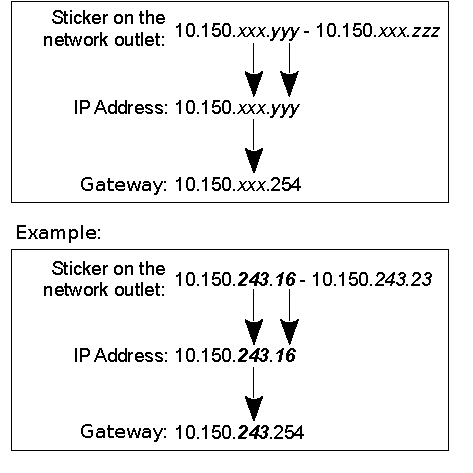
\includegraphics[width=\linewidth,keepaspectratio]{Bilder/IP_Gerneric_EN}
        \end{minipage}
\end{figure}


\clearpage
\enlargethispage{20pt}

\begin{figure}[h]
    \raggedleft
    \vspace{-20pt}
    
\includegraphics[height=1cm,keepaspectratio]{Bilder/Windows_logo}
    \vspace{-30pt}
\end{figure}

\subsubsection*{Step by step Windows settings}

\paragraph*{Windows 10}
\begin{enumerate}
    \item To open Control Panel click on the Windows button and choose \emph{Settings}.
    \item Click on \emph{Network and Internet}. Scroll down until \emph{Network and Sharing center} and select this point. Select in the left column \textit{change adapter settings}. If you cannot find this point, search for \emph{change adapter settings} in the toolbar.
    \item Click on \emph{Ethernet} and select \emph{Properties}.
\end{enumerate}
$\rightarrow$ Continue at point 5.

\begin{wrapfigure}[5]{R}{0.3\textwidth}
\centering
  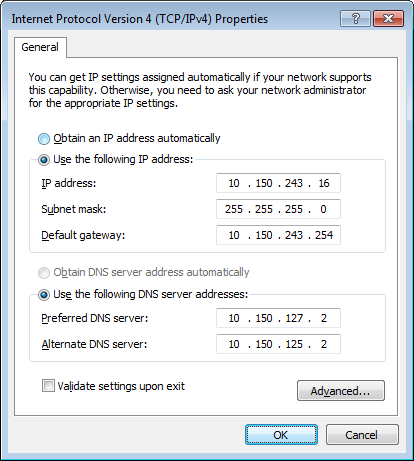
\includegraphics[width=0.3\textwidth]{Bilder/IP_Windows_EN}
%  \caption{Bildunterschrift}
\end{wrapfigure}

\paragraph*{Windows 8}
\begin{enumerate}	
	\item To open Control Panel press the Windows-Key and type Control Panel, then press ENTER.
    \item Click on \emph{Network and Internet} then on \emph{View network status and tasks}.
	\item Click on \emph{Change adapter settings} and then right click on the \emph{Local Area Connection} and select \emph{Properties}.
\end{enumerate}
$\rightarrow$ Continue at point 5.

\paragraph*{Windows 8/10}
\begin{enumerate}
    \setcounter{enumi}{4}
	\item Select \emph{Internet Protocol Verson 4 (TCP/IPv4)} (Windows 8/10) and click on \emph{Properties}.
    \item Now type in the IP address, the subnet mask (subnet prefix length), the Default gateway and the DNS Server. The DNS Server addresses are \textbf{10.150.127.2} and \textbf{10.150.125.2}, the Subnet mask is \textbf{255.255.255.0} (subnet prefix length is \textbf{24}). You can find your IP address on the sticker on the network outlet. Also you should have received a note containing your network settings with your rental agreement. If the sticker is unreadable or missing and you did not get the note containing the networksettings, please refer to the administration or visit one of our office hours.
    \item Click on Advanced and click on the DNS tab. Type \textbf{stusta.mhn.de} in the DNS suffix for this connection field.
	\item Confirm the settings with \emph{OK} and close the window.
\end{enumerate}
$\rightarrow$ Continue with the browser settings.


\pagebreak

\begin{figure}[t!]
    \raggedleft
    \vspace{-20pt}
    
\includegraphics[height=1cm,keepaspectratio]{Bilder/linux_logo_neu}
    \vspace{-30pt}
\end{figure}

\subsubsection*{Step by step Linux settings}
\begin{enumerate}
	\item Open the network configuration dialog by clicking on \emph{System} $\rightarrow$ \emph{Settings} $\rightarrow$ \emph{Network Settings}.
	\item Select your network card in the first tab (normally eth0) and click on \emph{Edit}.
	\item Click on the IPv4-Settings tab and change the method to \emph{Manually}.
	\item Under \emph{Addresses} click on Add.
      \begin{figure}[h!]
	\centering
		\begin{minipage}[c]{0.5\linewidth}
			\centering
			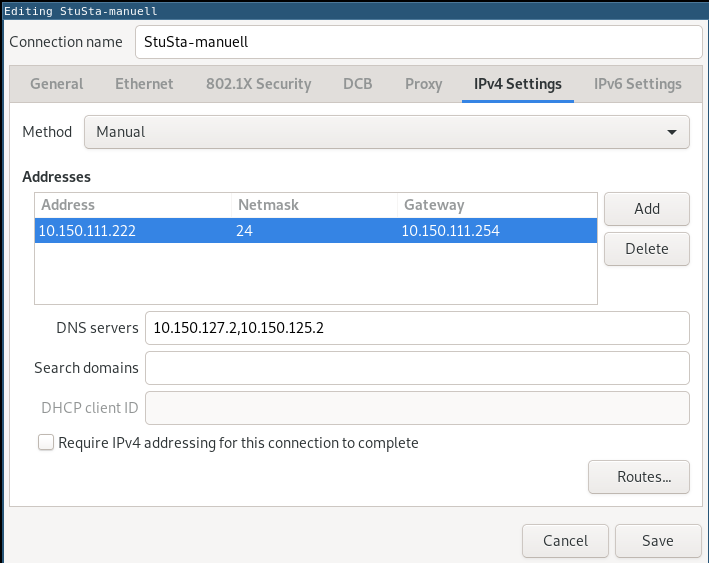
\includegraphics[width=0.9\linewidth,keepaspectratio]{Bilder/IP_Ubuntu_neu}
%			\caption{Beispielhafte Netzwerkeinstellungen unter Ubuntu Linux}
			\vspace{-15pt}
		\end{minipage}
	\end{figure}
  \item Now enter the IP address, the subnet mask, the gateway, the DNS and the search domain. The DNS server addresses are \textbf{10.150.127.2} and \textbf{10.150.125.2}, the search domain is \textbf{stusta.mhn.de} and the subnet mask is \textbf{255.255.255.0}. You can find your IP address on the sticker on the network outlet. Also you should have received a note containing your networksettings with your rental agreement. If the sticker is unreadable or missing and you did not get the note containing the networksettings, please refer to the administration or visit one of our office hours. Confirm the settings with \emph{OK} and close the window.
\end{enumerate}

\paragraph*{Global proxy settings} ~\\
\\
You can define a global proxy server in Linux so that you don't have to configure it for each browser individually.
\begin{enumerate}
	\item Open the network proxy settings by clicking on \emph{System} $\rightarrow$ \emph{Settings} $\rightarrow$ \emph{Network Proxy}.
    \item At the bottom of the window, mark the automatic proxy configuration box and enter the auto-configuration URL: \url{http://wpad.stusta.mhn.de/proxy.pac}. Close the window to save the settings.
\end{enumerate}



\newpage
\enlargethispage{20pt}

\begin{figure}[t!]
    \raggedleft
    \vspace{-20pt}
    
\includegraphics[height=1cm,keepaspectratio]{Bilder/apple_logo_neu}
    \vspace{-20pt}
\end{figure}
\subsubsection*{Step by step MacOS settings}
\begin{enumerate}
	\item Click on the \emph{Apple logo} (top left) and select \emph{System Preferences} $\rightarrow$ \emph{Network}.
	\item Select the \emph{Ethernet} connection.
	\item Set the \emph{Configure IPv4} drop-down box to \emph{Manually}.
	\item Now type in the IP address, the subnet mask, the gateway, the DNS and the search domain. The DNS server addresses are \textbf{10.142.0.2} and \textbf{10.142.0.3}, the search domain is \textbf{stusta.mhn.de} and the subnet mask is \textbf{255.255.255.0}. You can find your IP address on the sticker on the network outlet. Also you should have received a note containing your networksettings with your rental agreement. If the sticker is unreadable or missing and you did not get the note containing the networksettings, please refer to the administration or visit one of our office hours. Confirm the settings with \emph{Apply}.
      \begin{figure}[h!]
      \centering
%      \vspace{-5pt}
        \begin{minipage}[c]{0.60\linewidth}
          \centering
          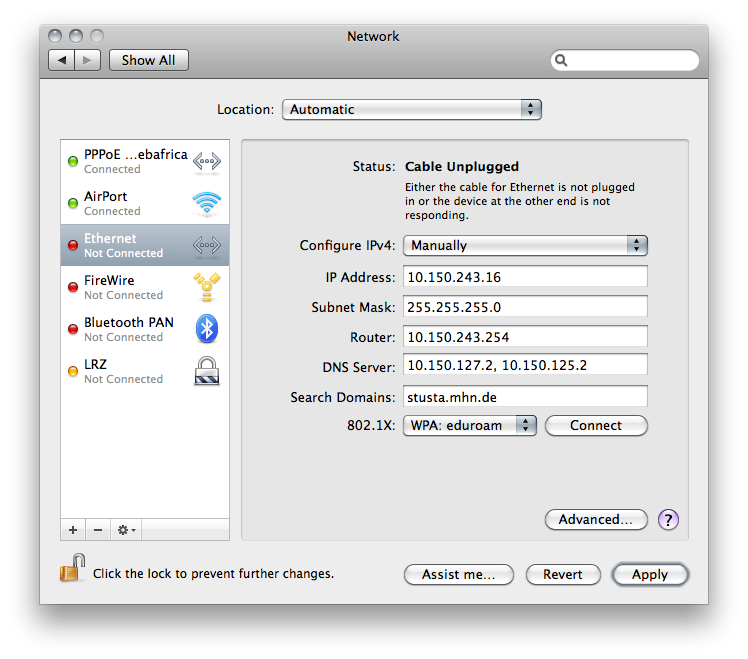
\includegraphics[width=0.9\linewidth,keepaspectratio]{Bilder/IP_Mac_EN}
%          \caption{Beispielhafte Netzwerkeinstellungen unter Mac OS~X}
        \end{minipage}
      \vspace{-20pt}
      \end{figure}
\end{enumerate}

\paragraph*{Global proxy settings}~\\
\\
You can define a global proxy server in MacOS so that you don't have to configure it for each browser individually. Firefox, however, still needs an individual configuration (see Browser settings).
\begin{enumerate}
	\item Click on \emph{Advanced} and select the \emph{Proxies} tab.
	\item Mark the checkbox next to \emph{Automatic Proxy Configuration} and type in the URL \url{http://wpad.stusta.mhn.de/proxy.pac}\ . Click on \emph{OK} and select \emph{Apply} one more time. You can now close System Preferences.
\end{enumerate}

\newpage

\section*{Proxy configuration in the browser (just non members)}

\begin{wrapfigure}{r}{0.5\textwidth}
	\vspace{-40pt}
	\begin{center}
		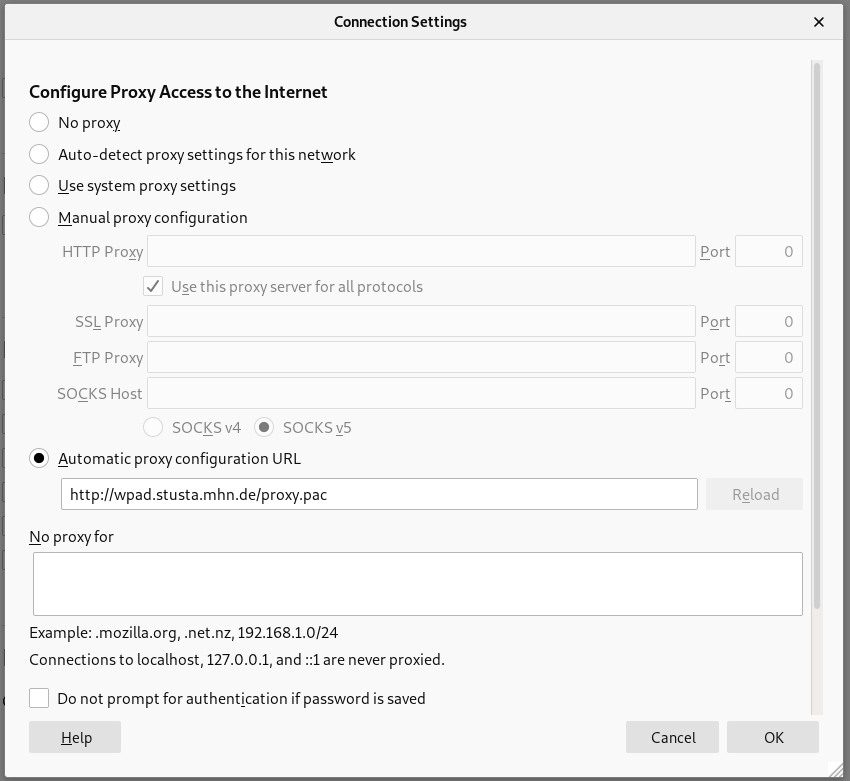
\includegraphics[width=0.5\textwidth,keepaspectratio]{Bilder/firefox_en_stusta}
	\end{center}
	%  \vspace{-20pt}
%	\caption{Eintragen des Proxyskripts in Mozilla Firefox}
	%  \vspace{-10pt}
\end{wrapfigure}

\subsection*{
\includegraphics[height=1.2cm,keepaspectratio]{Bilder/Firefox_35_logo} Mozilla Firefox}
\begin{enumerate}
	\item Click on the three stripes in the top right corner. Then choose \emph{Settings}.
	\item Scroll until \emph{Connection settings} and select this point.
	\item Mark the setting \emph{Automatic proxy configuration address} and use \\ \url{http://wpad.stusta.mhn.de/proxy.pac} as the Automatic proxy configuration URL.
	\item Confirm with \emph{OK}.\\
	\\
	\\
\end{enumerate}



\subsection*{
\includegraphics[height=1.2cm,keepaspectratio]{Bilder/Chrome_2011_logo} Google Chrome}
\begin{enumerate}
	\item Start Chrome.
	\item Click on the three stripes in the top right corner. Then choose \emph{Preferences}.
	\item Click on \emph{Advanced settings}.
	\item Click on \emph{open proxy settings of the computer}.
	\\
	\\
\end{enumerate}
$\rightarrow$ Continue at point 5 under Microsoft Edge.

\newpage
\begin{wrapfigure}{r}{0.5\textwidth}
	%  \vspace{-20pt}
	\begin{center}
		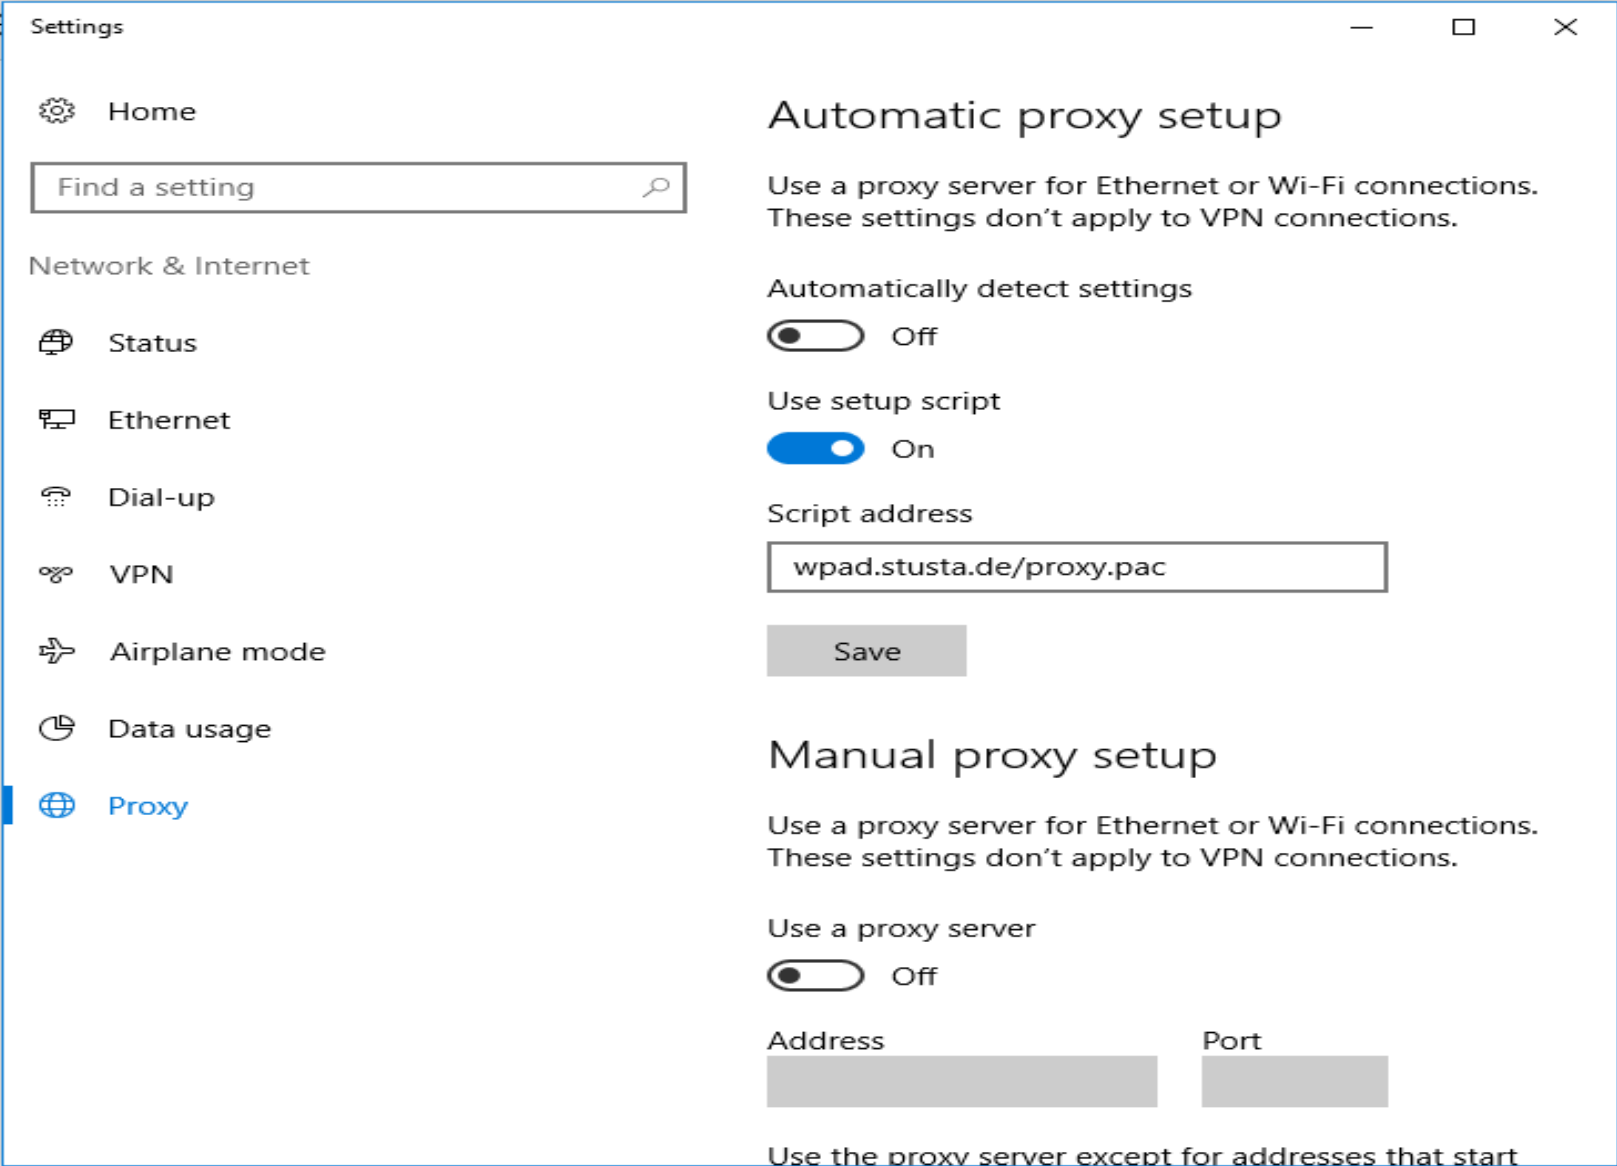
\includegraphics[width=0.5\textwidth,keepaspectratio]{Bilder/Proxy_Edge_EN}
	\end{center}
	%  \vspace{-20pt}
%	\caption{Configuring the proxy script in Microsoft Edge}
	%  \vspace{-10pt}
\end{wrapfigure}

\subsection*{
\includegraphics[height=1.2cm,keepaspectratio]{Bilder/Mcrosoft_Edge_logo} Microsoft Edge}
\begin{enumerate}
	\item Start Microsoft Edge.
	\item Click on the 3 overlapping stripes on the upper right corner and select \emph{Settings}.
	\item Select the button \emph{Advanced settings}.
	\item Click at \emph{Open proxy settings}.
	\item Deactive the option \emph{Autodetect the proxy settings}.
	\item Choose \emph{use setup-script} and enter the following url at address: \\ \url{http://wpad.stusta.mhn.de/proxy.pac}.
	\item Select save and close the windows.
\end{enumerate}
\end{document}
